\section{Planes}

\begin{outcome}
  \begin{enumerate}
  \item Find the vector and parametric equations of a plane in $\R^n$.
  \item Find the normal and general equations of a plane in $\R^3$.
  \item Find the intersection of two planes, or of a line and a plane.
  \item Find the angle between two planes, or between a line and a plane.
  \item Find the shortest distance between a point and a plane.
  \end{enumerate}
\end{outcome}

Much like the above discussion with lines, vectors can be used to
determine planes in $\R^n$. Consider a point $P$ and two direction
vectors $\vect{d}$ and $\vect{e}$ that are not parallel to each
other. Then there is a unique plane passing through $P$ and containing
$\vect{d}$ and $\vect{e}$:
\begin{center}
  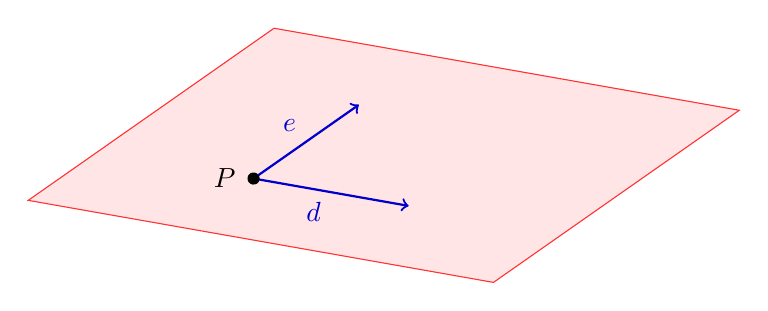
\begin{tikzpicture}[rotate=-10]
    \filldraw[draw=red!80,fill=red!10](-2,0,-5) -- (4,0,-5) -- (4,0,2) -- (-2,0,2) -- cycle;
    \draw[->,thick,blue!80!black](0,0,0) -- node[below left] {$\vect{d}$} (2,0,0);
    \draw[->,thick,blue!80!black](0,0,0) -- node[above left] {$\vect{e}$} (0,0,-3);
    \fill (0,0) circle [radius=2.2pt] node [left=3pt] {$P$};
  \end{tikzpicture}
\end{center}
The plane is infinite in each direction, although in the picture, we
have only shown a small part of it. If $\vect{p}$ is the position
vector of $P$ and $\vect{q}$ is the position vector of some other
point in the plane, we have
\begin{equation*}
  \vect{q} = \vect{p} + t\,\vect{d} + s\,\vect{e}
\end{equation*}
for some real numbers $t$ and $s$. This is called the \textbf{vector
  equation}%
\index{vector equation!of a plane}\index{plane!vector equation} of the
plane.

\begin{definition}{Vector equation of a plane}{vector-equation-of-plane}
  Let $\vect{p}$ be a vector and let $\vect{d},\vect{e}$ be non-zero,
  non-parallel vectors. Then
  \begin{equation*}
    \vect{q} = \vect{p} + t\,\vect{d} + s\,\vect{e}
  \end{equation*}
  is the \textbf{vector equation}%
  \index{vector equation!of a plane}\index{plane!vector equation} of a
  plane.
\end{definition}

The vector equation of a plane can also be written in
\textbf{component form}%
\index{vector equation!of a plane!component form}%
\index{component form!plane}\index{plane!component form}
\begin{equation*}
  \begin{mymatrix}{c} x_1 \\ x_2 \\ \vdots \\ x_n \end{mymatrix}
  = \begin{mymatrix}{c} p_1 \\ p_2 \\ \vdots \\ p_n \end{mymatrix}
  + t \begin{mymatrix}{r} d_1 \\ d_2 \\ \vdots \\ d_n \end{mymatrix},
  + s \begin{mymatrix}{r} e_1 \\ e_2 \\ \vdots \\ e_n \end{mymatrix}
\end{equation*}
and in \textbf{parametric form}
\begin{equation*}
  \begin{array}{c@{~}c@{~}c}
    x_1 &=& p_1 + t\,d_1 + s\,e_1, \\
    x_2 &=& p_2 + t\,d_2 + s\,e_2, \\
        &\vdots&             \\
    x_n &=& p_n + t\,d_n + s\,e_n.
  \end{array}
\end{equation*}
The latter set of equations are also called the \textbf{parametric
  equations}%
\index{parametric equations!of a plane}%
\index{plane!parametric equations} of the plane.

\begin{example}{Vector and parametric equations}{plane-from-three-points}
  Find vector and parametric equations for the plane through the
  points $P = (1,2,0,0)$, $Q = (2,2,0,1)$, and $R = (0,1,1,0)$.
\end{example}

\begin{solution}
  We can use $P$ as the base point and $\longvect{PQ}$ and
  $\longvect{PR}$ as the direction vectors. We have
  \begin{equation*}
    \longvect{PQ} =
    \begin{mymatrix}{c} 2\\2\\0\\1 \end{mymatrix}
    - \begin{mymatrix}{c} 1\\2\\0\\0 \end{mymatrix}
    = \begin{mymatrix}{c} 1\\0\\0\\1 \end{mymatrix}
    \quad\mbox{and}\quad
    \longvect{PR} =
    \begin{mymatrix}{c} 0\\1\\1\\0 \end{mymatrix}
    - \begin{mymatrix}{c} 1\\2\\0\\0 \end{mymatrix}
    = \begin{mymatrix}{c} -1\\-1\\1\\0 \end{mymatrix}.
  \end{equation*}
  Therefore the vector equation is
  \begin{equation*}
    \begin{mymatrix}{c} x\\y\\z\\w \end{mymatrix}
    = \begin{mymatrix}{c} 1\\2\\0\\0 \end{mymatrix}
    + t\,\begin{mymatrix}{c} 1\\0\\0\\1 \end{mymatrix}
    + s\,\begin{mymatrix}{c} -1\\-1\\1\\0 \end{mymatrix}.
  \end{equation*}
  We can also write this as a system of parametric equations:
  \begin{equation*}
    \begin{array}{c@{~}c@{~}l}
      x &=& 1 + t - s, \\
      y &=& 2 - s, \\
      z &=& s, \\
      w &=& t.
    \end{array}
  \end{equation*}
\end{solution}

Note that the vector and parametric equations of a plane are not
unique. For example, in Example~\ref{exa:plane-from-three-points}, we
could have equally used $Q$ or $R$ as the base point, and/or used
$\longvect{QR}$ as one of the direction vectors. In each case we would
have obtained a different equation for the same plane.

\begin{example}{Determine whether a point is on a plane}{point-on-plane-parametric}
  Determine whether the point $S=(4,4,-2,1)$ lies on the plane through
  the points $P = (1,2,0,0)$, $R = (2,2,0,1)$, and
  $Q = (0,1,1,0)$.
\end{example}

\begin{solution}
  We already found the parametric equations for this plane in
  Example~\ref{exa:plane-from-three-points}. To determine whether the
  point $S=(4,4,-2,1)$ lies on this plane, we must substitute its
  coordinates into the parametric equations:
  \begin{equation*}
    \begin{array}{r@{~}c@{~}l}
      4 &=& 1 + t - s, \\
      4 &=& 2 - s, \\
      -2 &=& s, \\
      1 &=& t.
    \end{array}
  \end{equation*}
  This is a system of linear equations. We solve it to find that it
  has the unique solution $(t,s) = (1,-2)$. Therefore, the point $S$
  lies on the given plane, and more specifically, it is the point that
  corresponds to the parameters $t=1$ and $s=-2$.
\end{solution}

In the special case of 3 dimensions, a plane can also be described by a
point and a normal vector. A \textbf{normal vector}%
\index{normal vector of a plane}\index{vector!normal vector}%
\index{plane!normal vector} of a plane is a vector that is
perpendicular to the plane.
\begin{center}
  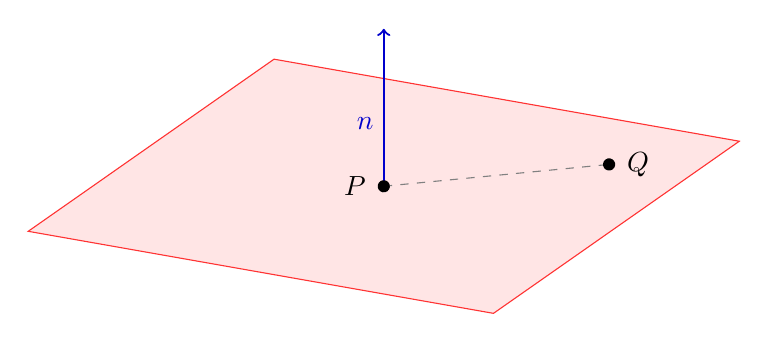
\begin{tikzpicture}[rotate=-10]
    \filldraw[draw=red!80,fill=red!10](-3,0,-3.5) -- (3,0,-3.5) -- (3,0,3.5) -- (-3,0,3.5) -- cycle;
    \draw[->,thick,blue!80!black](0,0,0) -- node[left, pos=0.4] {$\vect{n}$} (100:2);
    \draw[dashed,gray]((0,0,0) -- (2,0,-2);
    \fill (0,0,0) circle [radius=2.2pt] node [left=3pt] {$P$};
    \fill (2,0,-2) circle [radius=2.2pt] node [right=3pt] {$Q$};
  \end{tikzpicture}
\end{center}
Given a non-zero vector $\vect{n}$ in $\R^3$ and a point $P$, there
exists a unique plane that contains $P$ and has $\vect{n}$ as a normal
vector. We wish to find an equation for this plane. If $Q$ is an
arbitrary point on the plane, then by definition, the normal vector is
orthogonal to the vector $\longvect{PQ}$. Writing this as a formula,
we have $\vect{n} \dotprod \longvect{PQ} = 0$. If $\vect{p}$ and
$\vect{q}$ are the position vectors of $P$ and $Q$, respectively, we
have $\longvect{PQ} = \vect{q}-\vect{p}$, and therefore the equation
of the plane can be written as
\begin{equation*}
  \vect{n} \dotprod (\vect{q}-\vect{p}) = 0,
\end{equation*}
or equivalently,
\begin{equation*}
  \vect{n} \dotprod \vect{q} = \vect{n} \dotprod \vect{p}.
\end{equation*}
This is called the \textbf{normal equation} of the plane. Note that in
this equation, $\vect{n}$ and $\vect{p}$ are given and fixed, whereas
$\vect{q}$ is a variable ranging over the position vectors of all
points on the plane.

\begin{definition}{Normal equation of a plane in $\R^3$}{normal-equation-plane}
  Let $\vect{n}$ be a non-zero vector in $\R^3$, and let $P$ be a
  point with position vector $p$. Then there is a unique plane through
  $P$ with normal vector $\vect{n}$. It is described by the equation
  \begin{equation*}
    \vect{n} \dotprod \vect{q} = \vect{n} \dotprod \vect{p}.
  \end{equation*}
  This equation is called the \textbf{normal
    equation}\index{plane!normal equation}%
  \index{plane!normal equation}\index{normal equation of a plane} of
  the plane.
\end{definition}

\begin{example}{Finding the normal equation of a plane}{normal-equation}
  Find the normal equation of the plane through the point $P=(1,3,0)$
  and orthogonal to $\vect{n}=\mat{2,1,1}^T$.
\end{example}

\begin{solution}
  Let $\vect{p}=\mat{1,3,0}^T$ be the position vector of $P$, and let
  $\vect{q}=\mat{x,y,z}^T$ be the position vector of some arbitrary
  point $Q$ in the plane. The normal equation is
  $\vect{n} \dotprod \vect{q} = \vect{n} \dotprod \vect{p}$, which we
  can write in component form:
  \begin{equation*}
    \begin{mymatrix}{c}2\\1\\1\end{mymatrix}
    \dotprod
    \begin{mymatrix}{c}x\\y\\z\end{mymatrix}
    =
    \begin{mymatrix}{c}2\\1\\1\end{mymatrix}
    \dotprod
    \begin{mymatrix}{c}1\\3\\0\end{mymatrix}.
  \end{equation*}
  We can pre-compute the dot product on the right-hand side:
  $\vect{n} \dotprod \vect{p} = 1(2)+3(1)=0(1) = 5$. Therefore, the
  normal equation can also be written as
  \begin{equation*}
    \begin{mymatrix}{c}2\\1\\1\end{mymatrix}
    \dotprod
    \begin{mymatrix}{c}x\\y\\z\end{mymatrix}
    = 5.
  \end{equation*}
\end{solution}

Notice that the last equation in Example~\ref{exa:normal-equation} can
also be written in the form
\begin{equation*}
  2x + y + z = 5.
\end{equation*}
This last form is called the \textbf{general equation} of the plane.

\begin{definition}{General equation of a plane in $\R^3$}{general-equation-plane}
  Let $\vect{n} = \mat{a,b,c}^T$ be the normal vector for a plane that
  contains the point $P = (x_0, y_0, z_0)$. The \textbf{general
    equation}\index{plane!general equation}%
  \index{general equation of a plane} of the plane is given by
  \begin{equation*}
    ax + by + cz = d,
  \end{equation*}
  where $a,b,c,d \in \R$ and $d = ax_0 + by_0 + cz_0$.
\end{definition}

\begin{example}{Normal and general equations}{normal-from-three-points}
  Find normal and general equations for the plane through the points
  $P = (0,1,3)$, $Q=(2,-1,0)$, and $R=(1,2,2)$.
\end{example}

\begin{solution}
  We first need to find a normal vector for the plane. Since the
  normal vector must be perpendicular to the plane, it must be
  orthogonal to both $\longvect{PQ}$ and $\longvect{PR}$. We can
  therefore use the cross product to compute a normal vector for the
  plane:
  \begin{equation*}
    \vect{n}
    ~=~
    \longvect{PQ} \times \longvect{PR}
    ~=~
    \begin{mymatrix}{r} 2 \\ -2 \\ -3 \end{mymatrix}
    \times
    \begin{mymatrix}{r} 1 \\ 1 \\ -1 \end{mymatrix}
    ~=~
    \begin{mymatrix}{r} 5 \\ -1 \\ 4 \end{mymatrix}.
  \end{equation*}
  \begin{center}
    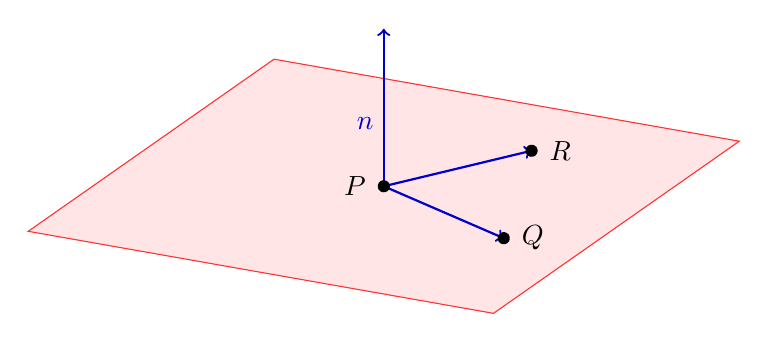
\begin{tikzpicture}[rotate=-10]
      \filldraw[draw=red!80,fill=red!10](-3,0,-3.5) -- (3,0,-3.5) -- (3,0,3.5) -- (-3,0,3.5) -- cycle;
      \draw[->,thick,blue!80!black](0,0,0) -- node[left, pos=0.4] {$\vect{n}$} (100:2);
      \draw[->,thick,blue!80!black]((0,0,0) -- (2,0,1);
      \draw[->,thick,blue!80!black]((0,0,0) -- (1,0,-2);
      \fill (0,0,0) circle [radius=2.2pt] node [left=3pt] {$P$};
      \fill (2,0,1) circle [radius=2.2pt] node [right=3pt] {$Q$};
      \fill (1,0,-2) circle [radius=2.2pt] node [right=3pt] {$R$};
    \end{tikzpicture}
  \end{center}
  Now we can easily obtain the normal equation from any point on the
  plane (say $P$) and the normal vector we just calculated:
  \begin{equation*}
    \begin{mymatrix}{r} 5 \\ -1 \\ 4 \end{mymatrix}
    \dotprod
    \begin{mymatrix}{r} x \\ y \\ z \end{mymatrix}
    =
    \begin{mymatrix}{r} 5 \\ -1 \\ 4 \end{mymatrix}
    \dotprod
    \begin{mymatrix}{r} 0 \\ 1 \\ 3 \end{mymatrix}
  \end{equation*}
  We get the general equation by computing the dot products on the
  left- and right-hand sides:
  \begin{equation*}
    5x - y + 4z = 11.
  \end{equation*}
  It is worthwhile to double-check the answer by substituting each of
  the three original points $P$, $Q$, and $R$ into this equation.
  For example, for $Q=(2,-1,0)$, we obtain $5(2)-(-1)+4(0)$, which is
  indeed $11$.
\end{solution}

\begin{example}{Find the normal vector of a plane}{find-normal}
  Find a normal vector for the plane $2x+3y-z=7$.
\end{example}

\begin{solution}
  The general equation $2x+3y-z=7$ can be rewritten as a normal
  equation
  \begin{equation*}
    \begin{mymatrix}{c} 2\\3\\7 \end{mymatrix}
    \dotprod
    \begin{mymatrix}{c} x\\y\\z \end{mymatrix}
    = 7.
  \end{equation*}
  Therefore,
  \begin{equation*}
    \vect{n} = \begin{mymatrix}{c} 2\\3\\7 \end{mymatrix}
  \end{equation*}
  is a normal vector for the plane.
\end{solution}

\begin{example}{Determine whether a point is on a plane}{point-plane-normal}
  Let $\vect{n} = \mat{1,2,3}^T$ be the normal vector for a plane
  which contains the point $P = (2,1,4)$. Determine if the point
  $Q = (5,4,1)$ is in this plane.
\end{example}

\begin{solution}
  By Definition~\ref{def:normal-equation-plane}, $Q$ is a point in the
  plane if and only if
  \begin{equation*}
    \vect{n} \dotprod \vect{q} = \vect{n} \dotprod \vect{p},
  \end{equation*}
  where $\vect{p}$ and $\vect{q}$ are the position vectors of $P$ and
  $Q$, respectively.  Given $\vect{n}$, $P$, and $Q$ as above, this
  equation becomes
  \begin{equation*}
    \begin{mymatrix}{r} 1 \\ 2 \\ 3 \end{mymatrix}
    \dotprod
    \begin{mymatrix}{r} 5 \\ 4 \\ 1 \end{mymatrix}
    ~=~
    \begin{mymatrix}{r} 1 \\ 2 \\ 3 \end{mymatrix}
    \dotprod
    \begin{mymatrix}{r} 2 \\ 1 \\ 4 \end{mymatrix}.
  \end{equation*}
Since both sides of the equation are equal to $16$, the equation is
  true. So the point $Q$ is indeed in the plane determined by
  $\vect{n}$ and $P$.
\end{solution}

\begin{example}{Vector equation from normal equation}{vector-from-normal}
  Find a vector equation for the plane $x+3y-2z=7$.
\end{example}

\begin{solution}
  This is the same thing as finding the general solution of a system
  of one linear equation in 3 variables. Since there is only a single
  equation $x+3y-2z=7$, it is already in {\ef}. The variables
  $y$ and $z$ are free, so we set them equal to parameters: $z=t$ and
  $y=s$. The variable $x$ is a pivot variable, and we get
  $x=7+2t-3s$. So the general solution of the equation is
  \begin{equation*}
    \begin{mymatrix}{c} x\\y\\z \end{mymatrix}
    = \begin{mymatrix}{r} 7\\0\\0 \end{mymatrix}
    + t\,\begin{mymatrix}{r} 2\\0\\1 \end{mymatrix}
    + s\,\begin{mymatrix}{r} -3\\1\\0 \end{mymatrix}.
  \end{equation*}
  This is also a vector equation for the plane.
\end{solution}

\begin{example}{Intersection of two planes}{intersection-planes}
  Find the intersection of the planes $x-2y+z=0$ and
  $2x-3y-z=4$.%
  \index{intersection!of two planes}
\end{example}

\begin{solution}
  Finding the intersection means finding all of the points $(x,y,z)$
  that are on both planes simultaneously. This is the same as solving
  the system of equations
  \begin{eqnarray*}
    x-2y+z &=& 0, \\
    2x-3y-z &=& 4.
  \end{eqnarray*}
  We solve the system by Gauss-Jordan elimination:
  \begin{equation*}
    \begin{mymatrix}{ccc|c}
      1 & -2 & 1 & 0 \\
      2 & -3 & -1 & 4
    \end{mymatrix}
    \stackrel{R_2\rowop R_2-2R_1}{\sim}
    \begin{mymatrix}{ccc|c}
      1 & -2 & 1 & 0 \\
      0 & 1 & -3 & 4
    \end{mymatrix}
    \stackrel{R_1\rowop R_1+2R_2}{\sim}
    \begin{mymatrix}{ccc|c}
      1 & 0 & -5 & 8 \\
      0 & 1 & -3 & 4
    \end{mymatrix}.
  \end{equation*}
  Therefore, the general solution is
  \begin{equation*}
    \begin{mymatrix}{c} x\\y\\z \end{mymatrix}
    =
    \begin{mymatrix}{c} 8\\4\\0 \end{mymatrix}
    + t\,\begin{mymatrix}{c} 5\\3\\1 \end{mymatrix},
  \end{equation*}
  where $t$ is a parameter. This is the parametric equation of a
  line. Therefore, the two planes intersect in a line. Specifically,
  the intersection is the line through the point $(8,4,0)$ with
  direction vector $\mat{5,3,1}^T$.
\end{solution}

\begin{example}{Intersection of a line and a plane}{intersection-line-plane}
  Find the intersection of the line
  \begin{equation*}
    \begin{mymatrix}{r} x \\ y \\ z \end{mymatrix}
    = \begin{mymatrix}{r} 1 \\ 2 \\ 0 \end{mymatrix}
    + t \begin{mymatrix}{r} -1 \\ 1 \\ 2 \end{mymatrix}
  \end{equation*}
  and the plane $2x+2y-z = 2$.%
  \index{intersection!of a line and a plane}
\end{example}

\begin{solution}
  Let us write
  \begin{equation*}
    \vect{p}=\begin{mymatrix}{c}1\\2\\0\end{mymatrix},
    \quad
    \vect{d}=\begin{mymatrix}{c}-1\\1\\2\end{mymatrix},
    \quad
    \vect{n}=\begin{mymatrix}{c}2\\2\\-1\end{mymatrix},
    \quad\mbox{and}\quad
    \vect{q}=\begin{mymatrix}{c}x\\y\\z\end{mymatrix}.
  \end{equation*}
  Then the equation of the line is $\vect{q}=\vect{p}+t\,\vect{d}$ and
  the equation of the plane is
  $\vect{n}\dotprod\vect{q}=2$. Substituting the first equation into
  the second one, we get $\vect{n}\dotprod(\vect{p}+t\,\vect{d}) = 2$.
  Using distributivity of the dot product, we can write this last
  equation as
  $\vect{n}\dotprod\vect{p} + t(\vect{n}\dotprod\vect{d}) = 2$.  By
  computing the dot products $\vect{n}\dotprod\vect{p}=6$ and
  $\vect{n}\dotprod\vect{d} = -2$, this equation simplifies to
  $6-2t=2$, or $t=2$. Therefore, the line intersects the plane when
  $t=2$, or at the point
  \begin{equation*}
    \begin{mymatrix}{r} x \\ y \\ z \end{mymatrix}
    = \begin{mymatrix}{r} 1 \\ 2 \\ 0 \end{mymatrix}
    + 2 \begin{mymatrix}{r} -1 \\ 1 \\ 2 \end{mymatrix}
    = \begin{mymatrix}{r} -1 \\ 4 \\ 4 \end{mymatrix}.
  \end{equation*}
  An alternative method is to directly substitute the parametric
  equation of the line, $x=1-t$, $y=2+t$, and $z=2t$, into the
  equation of the plane, $2x+2y-z = 2$. In this case, we get
  $2(1-t)+2(2+t)-(2t)=2$, which we can solve for $t$ to obtain $t=2$.
\end{solution}

The next few examples are concerned with calculating angles between
planes, angles between lines and planes, and finding the distance
between points and planes.

\begin{example}{Find the angle between two planes}{angle-planes}
  Find the angle between the planes $7x-y=5$ and $4x+3y+5z=3$.%
  \index{angle!between two planes}\index{plane!angle between}
\end{example}

\begin{solution}
  The angle between two planes is the same thing as the angle between
  their normal vectors.
  \begin{center}
    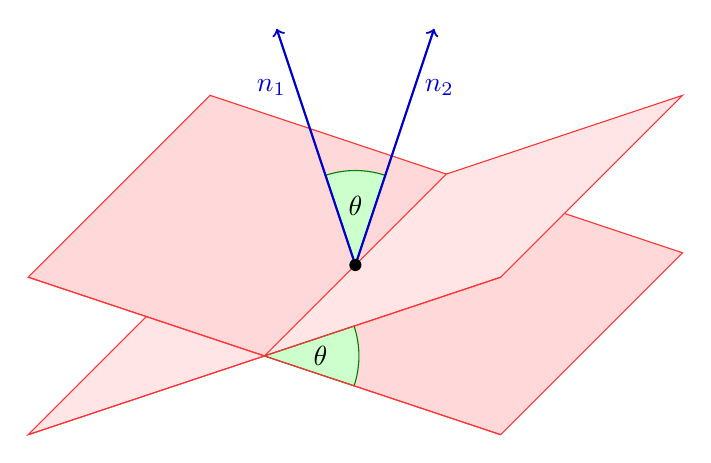
\begin{tikzpicture}
      \filldraw[draw=red!80,fill=red!10] (-3,-1,-3) -- (0,0,-3) -- (0,0,3) -- (-3,-1,3) -- cycle;
      \filldraw[draw=red!80,fill=red!15] (-3,1,-3) -- (3,-1,-3) -- (3,-1,3) -- (-3,1,3) -- cycle;
      \filldraw[draw=red!80,fill=red!10] (0,0,-3) -- (3,1,-3) -- (3,1,3) -- (0,0,3) -- cycle;
      \filldraw[fill=green!20,draw=green!50!black] (0,0,3) -- +(-18.4:12mm) arc (-18.4:18.4:12mm) -- cycle;
      \filldraw[fill=green!20,draw=green!50!black] (0,0,0) -- +(71.6:12mm) arc (71.6:108.4:12mm) -- cycle;
      \draw[red!80] (3,1,3) -- (-3,-1,3);
      \draw[red!80] (3,-1,3) -- (-3,1,3);
      \draw[->,thick,blue!80!black](0,0,0) -- node[left, near end] {$\vect{n}_1$} (-1,3,0);
      \draw[->,thick,blue!80!black](0,0,0) -- node[right, near end] {$\vect{n}_2$} (1,3,0);
      \fill (0,0,0) circle [radius=2.2pt];
      \node at (0,0,0) [above=5mm] {$\theta$};
      \node at (0,0,3) [right=5mm] {$\theta$};
    \end{tikzpicture}
  \end{center}
  The normal vectors are $\vect{n}_1 = \mat{7,-1,0}^T$ and $\vect{n}_2
  = \mat{4,3,5}$. The angle between them is given by
    \begin{equation*}
    \cos\theta =
    \frac{\vect{n}_1\dotprod\vect{n}_2}{\norm{\vect{n}_1}\norm{\vect{n}_2}}
    = \frac{25}{50} = \frac{1}{2}.
  \end{equation*}
  Therefore, the angle is $\arccos(\frac{1}{2}) = \pi/3$, or 60 degrees.
\end{solution}

\begin{example}{Find the angle between a line and a plane}{angle-line-plane}
  Find the angle between the line
  \begin{equation*}
    \begin{mymatrix}{r} x \\ y \\ z \end{mymatrix}
    = \begin{mymatrix}{r} 1 \\ 2 \\ 0 \end{mymatrix}
    + t \begin{mymatrix}{r} 2 \\ -1 \\ -2 \end{mymatrix}
  \end{equation*}
  and the plane $2x+2y-z = 2$.%
  \index{angle!between line and plane}
\end{example}

\begin{solution}
  To get the angle $\theta$ between the plane and the line, we can
  compute the angle $\phi$ between the direction vector of the line
  and the normal vector of the plane, and then take
  $\theta = \frac{\pi}{2}-\phi$.
  \begin{center}
    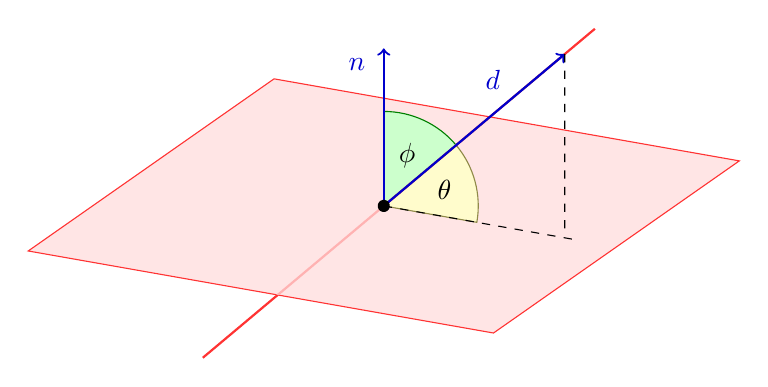
\begin{tikzpicture}[rotate=-10]
      \draw[thick, red!80] (50:-3) -- (0,0);
      \filldraw[draw=red!80,fill=red!10](-3,0,-3.5) -- (3,0,-3.5) -- (3,0,3.5) -- (-3,0,3.5) -- cycle;
      \filldraw[fill=yellow!20,draw=yellow!50!black] (0,0) -- (0:12mm) arc (0:50:12mm) -- cycle;
      \filldraw[fill=green!20,draw=green!50!black] (0,0) -- (50:12mm) arc (50:100:12mm) -- cycle;
      \draw[thick, red!80] (0,0) -- (50:3.5);
      \begin{scope}
        \clip (-3,0,-3.5) -- (3,0,-3.5) -- (3,0,3.5) -- (-3,0,3.5) -- cycle;
        \draw[thick, red!30] (50:-3) -- (0,0);
      \end{scope}
      \draw[->,thick,blue!80!black](0,0,0) -- node[left=3pt, pos=0.9] {$\vect{n}$} (100:2);
      \draw[->,thick,blue!80!black](0,0) -- node[above left, pos=0.7] {$\vect{d}$} (50:3);
      \draw[dashed] (0,0,0) -- (2.5,0,0);
      \draw[dashed] (50:3) -- +(100:-2.3);
      \fill (0,0,0) circle [radius=2.2pt];
      \node at (25:8mm) {$\theta$};
      \node at (75:7mm) {$\phi$};
    \end{tikzpicture}
  \end{center}
  The direction vector of the line is $\mat{2,-1,-2}^T$ and the normal
  vector of the plane is $\mat{2,2,-1}$. We have 
  \begin{equation*}
    \cos\phi =
    \frac{\vect{n}\dotprod\vect{d}}{\norm{\vect{n}}\norm{\vect{d}}}
    = \frac{4}{9},
  \end{equation*}
  and therefore $\phi = \arccos(\frac{4}{9}) \approx 1.11$ radians. We
  have $\theta = \frac{\pi}{2} - \phi \approx 0.46$ radians, or about
  26.4 degrees.
\end{solution}

\begin{example}{Shortest distance from a point to a plane}{shortest-distance-plane}
  Find the shortest distance from the point $P = (3,2,3)$ to the plane
  given by $2x + y + 2z = 2$, and find the point $Q$ on the plane
  that is closest to $P$.%
  \index{distance!point to plane}\index{projection!point to plane}
\end{example}

\begin{solution}
  In this problem, we are going to use the projection of one vector
  onto another, which was introduced in
  Section~\ref{ssec:projections}.  Pick an arbitrary point $R$ on
  the plane. Then, it follows that
  \begin{equation*}
    \longvect{QP} = \proj_{\vect{n}}\,\longvect{RP}
  \end{equation*}
  and $\norm{\longvect{QP}}$ is the shortest distance from $P$ to the
  plane. Further, the position vector of the point $Q$ can be computed
  as $\vect{q} = \vect{p} - \longvect{QP}$, where $\vect{p}$ is the
  position vector of $P$.
  \begin{center}
    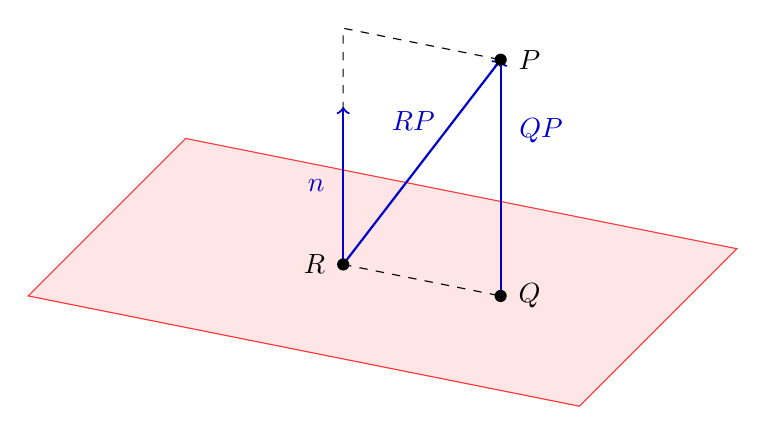
\begin{tikzpicture}[x={(1cm,-0.2cm)},y={(0.5cm,0.5cm)},z={(0cm,1cm)}]
      \filldraw[draw=red!80,fill=red!10](-3,-2,0) -- (4,-2,0) -- (4,2,0) -- (-3,2,0) -- cycle;
      \draw[dashed](0,0,0) -- (2,0,0) -- (2,0,3) -- (0,0,3) -- cycle;
      \draw[->,thick,blue!80!black](0,0,0) -- node[left=3pt] {$\vect{n}$} (0,0,2);
      \draw[->,thick,blue!80!black](0,0,0) -- node[left=3pt, pos=0.7] {$\longvect{RP}$} (2,0,3);
      \draw[->,thick,blue!80!black](2,0,0) -- node[right=3pt, pos=0.7] {$\longvect{QP}$} (2,0,3);
      \fill (0,0,0) circle [radius=2.2pt] node [left=3pt] {$R$};
      \fill (2,0,3) circle [radius=2.2pt] node [right=3pt] {$P$};
      \fill (2,0,0) circle [radius=2.2pt] node [right=3pt] {$Q$};
    \end{tikzpicture}
  \end{center}
  From the above scalar equation, we have that $\vect{n} =
  \begin{mysmallmatrix}{c} 2 \\ 1 \\ 2 \end{mysmallmatrix}$.  Now, choose any
  point on the plane, for example, $R = (1,0,0)$ (notice that this
  satisfies $2x+y+2z=2$).  Then,
  \begin{equation*}
    \longvect{RP} = \begin{mymatrix}{c} 3 \\ 2 \\ 3 \end{mymatrix}
    - \begin{mymatrix}{c} 1 \\ 0 \\ 0 \end{mymatrix} =
    \begin{mymatrix}{c} 2 \\ 2 \\ 3 \end{mymatrix}.
  \end{equation*}
  Next, compute $\longvect{QP} = \proj_{\vect{n}}\longvect{RP}$.
  \begin{equation*}
    \longvect{QP} ~=~ \proj_{\vect{n}}\longvect{RP} 
    ~=~ \paren{\frac{ \longvect{RP} \dotprod \vect{n}}{\norm{\vect{n}} ^2}}\vect{n} 
    ~=~ \frac{12}{9} \begin{mymatrix}{r} 2 \\ 1 \\ 2 \end{mymatrix} 
    ~=~ \frac{4}{3} \begin{mymatrix}{r} 2 \\ 1 \\ 2 \end{mymatrix}.
  \end{equation*}
  Then, $\norm{\longvect{QP}} = 4$ so the shortest distance from $P$
  to the plane is $4$.  To find the point $Q$ on the plane that is
  closest to $P$, we have
  \begin{equation*}
    \vect{q} ~=~ \vect{p} - \longvect{QP} 
    ~=~ \begin{mymatrix}{r} 3 \\ 2 \\ 3 \end{mymatrix}
    -
    \frac{4}{3} \begin{mymatrix}{r} 2 \\ 1 \\ 2 \end{mymatrix} 
    ~=~
    \frac{1}{3}
    \begin{mymatrix}{r} 1 \\ 2 \\ 1 \end{mymatrix}.
  \end{equation*}
  Therefore, $Q = (\frac{1}{3},\frac{2}{3},\frac{1}{3})$.
\end{solution}
